\documentclass[tikz,border=10pt]{standalone}
\usepackage{amsmath}
\begin{document}
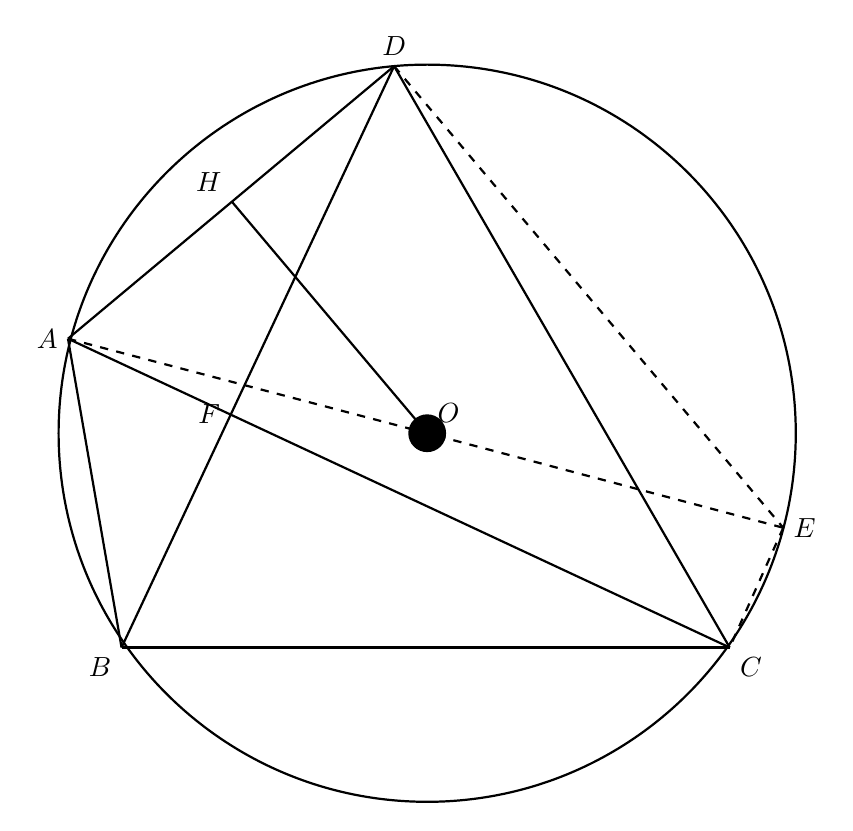
\begin{tikzpicture}[scale=0.02, line width=0.8pt]
  % circumcircle
  \draw (0,0) circle (234);

  % coordinates
  \coordinate (A) at (-228,60);
  \coordinate (B) at (-194,-136);
  \coordinate (C) at (192,-136);
  \coordinate (D) at (-21,233);
  \coordinate (E) at (226,-60);
  \coordinate (H) at (-124,147);
  \coordinate (O) at (0,0);
  \coordinate (F) at (-125,12);

  % solid edges
  \draw (A) -- (D);
  \draw (D) -- (B);
  \draw (D) -- (C);
  \draw (A) -- (C);
  \draw (A) -- (B);
  \draw (B) -- (C);
  \draw (H) -- (O);

  % dashed edges
  \draw[dashed] (A) -- (O) -- (E);
  \draw[dashed] (D) -- (E);
  \draw[dashed] (E) -- (C);

  % center point
  \fill (O) circle (12);

  % labels
  \node[above] at (D) {$D$};
  \node[above left] at (H) {$H$};
  \node[above right] at (O) {$O$};
  \node[left] at (A) {$A$};
  \node[below left] at (B) {$B$};
  \node[below right] at (C) {$C$};
  \node[right] at (E) {$E$};
  \node[left] at (F) {$F$};
\end{tikzpicture}
\end{document}
